\subsection{RQ2: What factors impact the difficulty of a conflict resolution?}
\textbf{***Q36 - Please rate how much each of these factor into the difficulty of resolving merge conflicts***}

%\begin{figure}[!t]
%\centering
%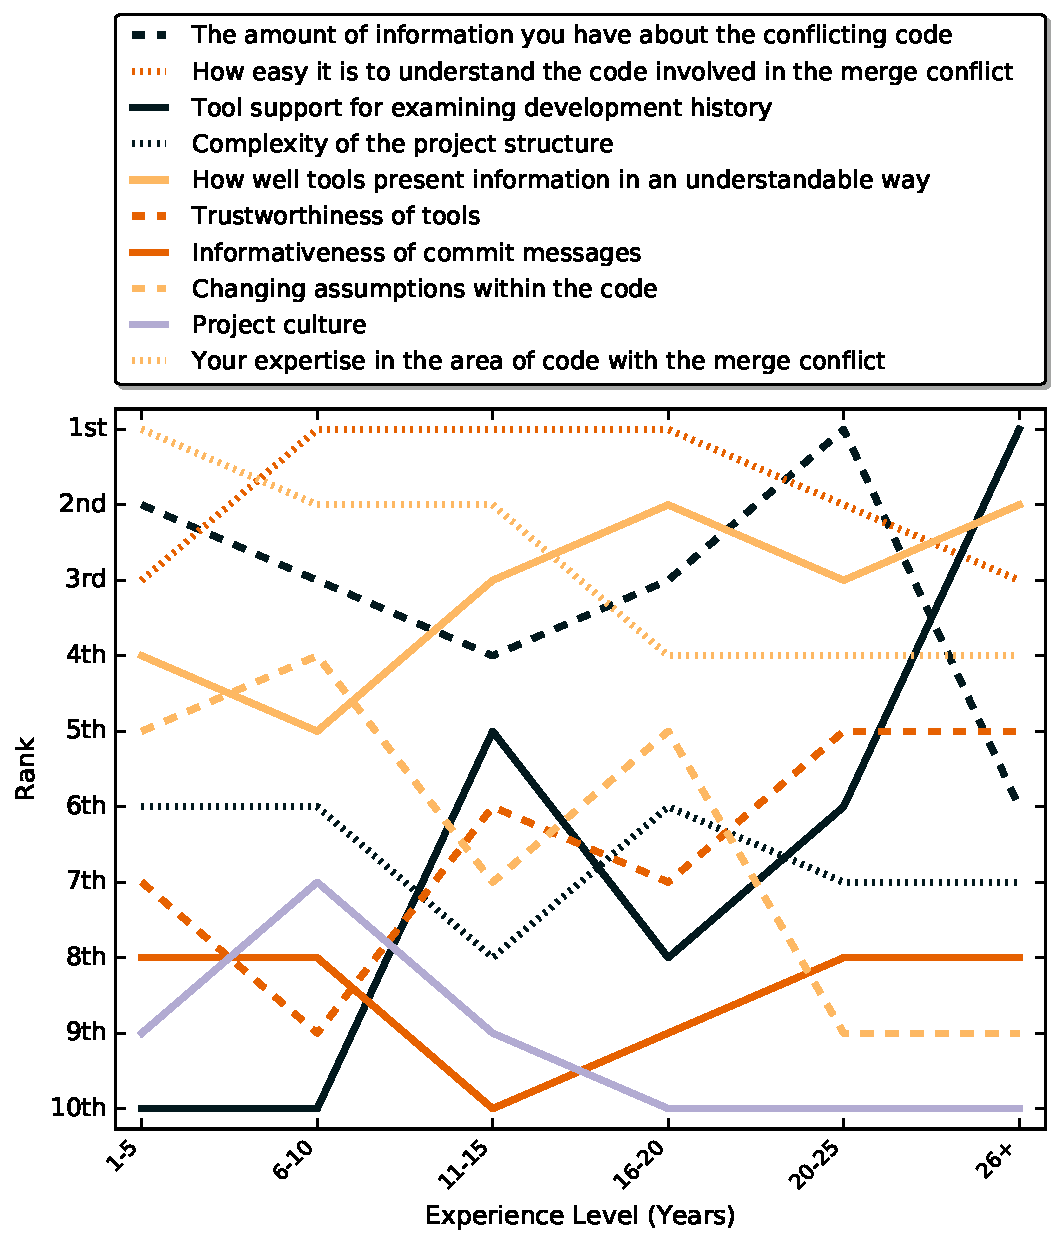
\includegraphics[width=2.5in]{ExpVsRankResDiff.pdf}
%\caption{The rank of factors of difficulty during merge conflict resolutions by experience level}
%\label{res_diff_rank}
%\end{figure}

These individual factors emerged through the interview processing via the method of card sorting previously described. Of 141 responses, Figure \ref{res_diff_rank} shows the rank of each factor where the rank 1 factors into the difficulty of resolving a merge conflict the most, and the rank 10 affects the difficulty of merge conflict resolution the least.

Some key factors to consider in Figure \ref{res_diff_rank}:
\begin{itemize}
\item \textbf{Tool support for examining development history}\\
This factor starts out ranked as the factor that least affects the difficulty of a merge conflict resolution in the group of least experienced respondants.
\item \textbf{Another key point}\\
***Explanation*** 
\end{itemize}

\textbf{***Tool support for examining development history from 10th to 1st***}\\
\textbf{***Expertise in the area of code becomes less important (1-4) ***}\\
\textbf{***Project Culture generally not important, especially with more experience***}\\
\textbf{***commit message informativeness lower than expected***}\\

%\begin{figure}[!t]
%\centering
%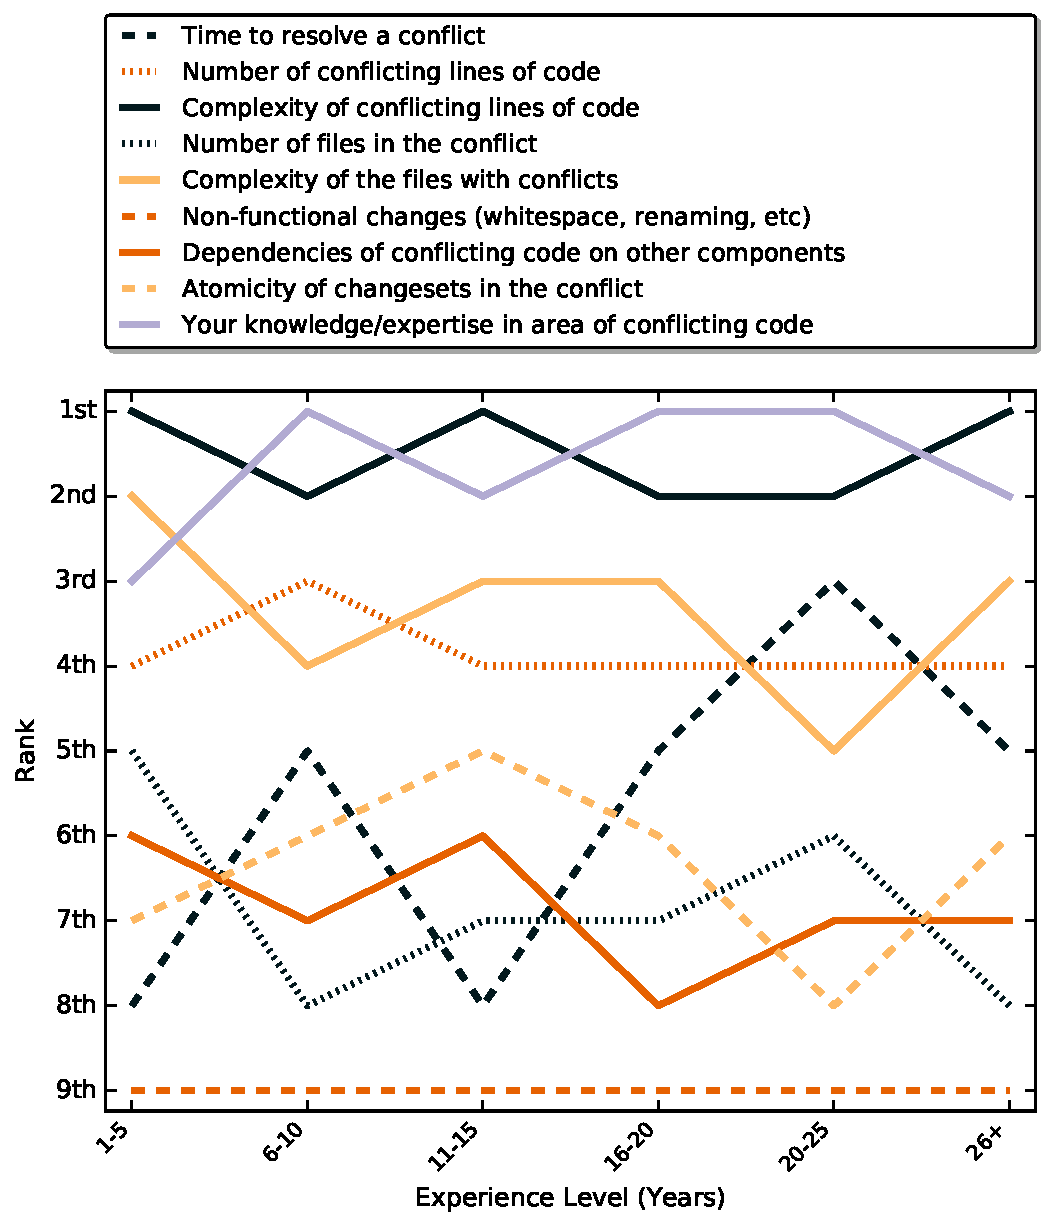
\includegraphics[width=2.5in]{ExpVsRankConDiff.pdf}
%\caption{Rank of difficult factors in merge conflicts by experience level}
%\label{con_diff_rank}
%\end{figure}